%GG
%Que Fait le projet
%Organisation du travail
%Découpage de l'archive (cmake)
%couverture de code

%Alienor
%main.c
%solveur
%valgrind

%ENSEMBLE
%Ce qui fonctionne/ ne fonctionne pas
%Difficultés rencontrées


%classe du document
\documentclass{report}

%importation des packages
\usepackage[utf8]{inputenc}
\usepackage[T1]{fontenc}
\usepackage[francais]{babel}
\usepackage{listings}
\usepackage{layout}
\usepackage[top = 4.5cm, bottom = 4.5cm, right = 3.5cm, left = 3.5cm]{geometry}
\usepackage{graphicx}
\usepackage{url}
\usepackage{verbatim}
\usepackage{moreverb}

%initialisation de la page de garde
\title{Projet de Programmation :\\ \bsc{rush hour} / \bsc{âne rouge}}
\author{IN400A1 - \bsc{Groupe 6}\\Aliénor \bsc{brabant}\\Abdoul \bsc{diallo}\\Gérard \bsc{lézé}\\{Manon \bsc{philippot}}}
\date{20 Avril 2016}

%configuration de la citation de code
\lstset{
language = C,
basicstyle = \scriptsize,
numbers = left,
numberstyle = \scriptsize,
numbersep = 7pt,
}

%début du rapport
\begin{document}

%page de garde et table des matières
\maketitle
\tableofcontents

%P1
\part{Le projet}

%P1C1
\chapter{Que fait le projet ?}
Dans de le cadre de l'UE ``Environnement de Développement et Projet de Programmation 1'' il nous a été donné comme projet la réalisation d'un jeu appelé \emph{Rush-Hour} et de son solveur. Ce jeu est un casse tête. La grille, ou aire de jeu, est un carré de 6 cases sur 6. Les pièces placées sur le jeu sont des véhicules. On distingue:
\begin{itemize}
\item Les voitures, qui occupent 2 cases adjacentes.
\item Les camions, qui occupent 3 cases adjacentes formant une ligne droite.
\item La voiture rouge, qui est aussi une voiture, mais qui se distingue des autres par le fait que c’est celle-là qu’il faut essayer de sortir de l’aire de jeu.
\end{itemize}

Le seul endroit où la voiture rouge peut sortir se trouve à droite de la case située en 3ème ligne et en 6ème colonne. Un véhicule ne peut se déplacer que sur une seule dimension, verticalement ou horizontalement, selon qu’il a été placé, respectivement, verticalement ou horizontalement. Il n’est pas permis d’enlever (ou de placer) un véhicule en cours de jeu. Le but du jeu est donc de faire sortir la voiture rouge de l’aire de jeu, en n’y effectuant que des déplacements légaux : c'est à dire un déplacement sur des cases libres sans passer outre d'autre véhicule.

Au cours du projet le cahier des charges évolue pour permettre d’étendre le \emph{Rush-Hour} et d’implémenter aussi le jeu de l’\emph{Âne-Rouge}, similaire au \emph{Rush-Hour} mais dont les pièces peuvent être de taille et de largeur toutes deux différentes de 1 et se déplacent à la fois horizontalement et verticalement. De plus les dimensions du plateaux sont de 4 cases sur 5. Le nouveau solveur devant résoudre les configurations de l'\emph{Âne-Rouge}.

Le projet sert de prétexte pour nous faire appréhender de manière ludique les nombreux outils utiles et/ou nécessaires au développement. Les outils de compilations \emph{Make} et \emph{CMake}. Les logiciels de gestions de version \emph{git} et \emph{svn}. L’outil de débogage \emph{gdb}. L’outil de recherche des fuites mémoires \emph{valgrind}. L’outil de couverture de code \emph{gcov}. Ainsi que l’importance des tests. Nous avons aussi pu nous confronté au mécanisme du travail en équipe et à l’organisation que cela demande.
%P1C2
\chapter{Description des fonctions implémentées}
\section{Fichier piece.c}
Le fichier piece.c implémente les fonctions nécéssaires à la création d'une pièce de jeu pouvant être utilisée pour les jeux de Rush Hour et d'Âne Rouge. Il est possible de réutiliser ce fichier source pour implémenter les pièces de jeux dont le fonctionnement est similaire.
\subsection{Structure pièce}
Une piece est modélisée par une structure C possédant six données membres :
\begin{itemize}
\item \emph{x} : abscisse du coin en bas à gauche de la pièce.
\item \emph{y} : ordonnée du coin en bas à gauche de la pièce.
\item \emph{width} : largeur de la pièce.
\item \emph{height} : hauteur de la pièce.
\item \emph{move\_x} : indique si la pièce est autorisée à bouger horizontalement.
\item \emph{move\_y} : indique si la pièce est autorisée à bouger verticalement.
\end{itemize}
\subsection{new\_piece}
La fonction \emph{new\_piece} crée une pièce en choisissant sa position sur le plateau de jeu, sa taille ainsi que ses capacités de mouvement. Elle consiste à allouer de la mémoire pour la structure \emph{piece} et à initialiser chaque donnée membre de la structure par l'argument correspondant passé en paramètre. Elle retourne la pièce en question. Le principe de cette fonction est utilisé pour implémenter la fonction \emph{new\_piece\_rh} permettant uniquement de créer une pièce de jeu pour Rush Hour.
\subsection{delete\_piece}
\label{del}
La fonction \emph{delete\_piece} supprime une pièce. Elle consiste à libérer la mémoire allouée à la pièce passée en paramètre en effectuant un \emph{free}. Elle ne retourne rien.
\subsection{copy\_piece}
\label{copy}
La fonction \emph{copy\_piece} copie la pièce passée en premier paramètre dans la pièce passée en second paramètre. On considère que la pièce copiée a déjà été initialisée avant l'appel à la fonction \emph{copy\_piece}. Elle consiste donc à uniquement copier les données membres de la pièce originale dans les données membres de la pièce copiée. Elle ne retourne rien.
\subsection{move\_piece}
La fonction \emph{move\_piece} bouge la pièce \emph{p} passée en premier paramètre, dans la direction \emph{dir} passée en second paramètre, d'une distance \emph{dist} passée en troisième paramètre. Si \emph{dir} vaut \emph{RIGHT}, alors l'abscisse \emph{x} de \emph{p} est incrémentée de \emph{dist}. Si \emph{dir} vaut \emph{LEFT}, alors l'abscisse \emph{x} de \emph{p} est décrémentée de \emph{dist}. Si \emph{dir} vaut \emph{UP}, alors l'ordonnée \emph{y} de \emph{p} est incrémentée de \emph{dist}. Si \emph{dir} vaut \emph{DOWN}, alors l'ordonnée \emph{y} de \emph{p} est décrémentée de \emph{dist}. Cette fonction ne retourne rien. Elle se contente uniquement de bouger la pièce, sans prendre en compte les mouvements invalides (mouvement en dehors du plateau, intersection de pièces, direction invalide). C'est l'implémentation de la fonction \emph{play\_move} du fichier source game.c qui s'en charge (cf. sous-section \ref{move}).
\subsection{intersect}
La fonction \emph{intersect} teste si les deux pièces passées en paramètre s'intersectent. Elle consiste à comparer les coordonnées de chaque cellule de la première pièce avec les coordonnées de chaque cellule de la seconde pièce. Elle retourne un bouléen, qui vaut \emph{true} si les deux pièces ont au moins une cellule en commun, et \emph{false} dans le cas contraire.
\subsection{Getteurs}
Les fonctions \emph{get\_x}, \emph{get\_y}, \emph{get\_height}, \emph{get\_width}, \emph{can\_move\_x} et \emph{can\_move\_y} sont des getteurs qui retournent respectivement l'abscisse \emph{x}, l'ordonnée \emph{y}, la hauteur \emph{height}, la largeur \emph{width}, le booléen \emph{move\_x} indiquant la capacité de mouvement horizontal et le booléen \emph{move\_y} indiquant la capacité de mouvement verticale de la pièce. Il existe également une fonction \emph{is\_horizontal} dont l'implémentation est similaire à celle de la fonction \emph{can\_move\_x}.
\section{Fichier game.c}
Le fichier game.c implémente les fonctions nécéssaires à la création d'un plateau de jeu, et à la gestion d'un jeu de Rush Hour et d'Ane Rouge. Il est possible de réutiliser ce fichier source pour implémenter des jeux dont le fonctionnement est similaire.
\subsection{Structure game}
Un jeu est modélisé par une structure C possédant cinq données membres :
\begin{itemize}
\item \emph{width} : largeur du plateau de jeu.
\item \emph{height} : hauteur du plateau de jeu.
\item \emph{nb\_pieces} : nombre de pièces sur le plateau de jeu.
\item \emph{nb\_moves} : nombre mouvement depuis le début du jeu.
\item \emph{pieces} : tableau de pièces.
\end{itemize}
\subsection{new\_game}
La fonction \emph{new\_game} crée un jeu en choisissant ses dimensions ainsi que la configuration initiale de celui-ci par l'intermédiaire d'un set de pièces. Elle consiste à allouer de la mémoire pour la structure \emph{game} et à initialiser chaque donnée membre de la structure par l'argument correspondant passé en paramètre. L'initialisation du tableau de pièces de la structure est assez particulière. Il faut d'abord allouer l'espace mémoire pour le tableau de pièces de la structure, puis copier chaque pièce du tableau fourni en paramètre dans le tableau \emph{pieces} de la structure par l'intermédiaire de la fonction \emph{copy\_piece} expliquée à la sous-section \ref{copy}. Cette fonction retourne le jeu en question. Le principe de cette fonction est utilisé pour implémenter la fonction \emph{new\_game\_hr} permettant uniquement de créer un jeu de Rush Hour.
\subsection{delete\_game}
La fonction \emph{delete\_game} supprime un jeu. Elle consiste à libérer la mémoire allouée au jeu passé en paramètre en supprimant dans un premier temps toutes les pièces du tableau de pièces par l'intermédiaire de la fonction \emph{delete\_piece} expliquée à la sous-section \ref{del}, puis en effectuant un \emph{free} sur le tableau et un \emph{free} sur le jeu en question. Elle ne retourne rien.
\subsection{copy\_game}
La fonction \emph{copy\_piece} copie le jeu passé en premier paramètre dans le jeu passé en second paramètre. On considère que le jeu copié a déjà été initialisé avant l'appel à la fonction \emph{copy\_game}. Elle consiste donc à uniquement copier les données membres du jeu original dans les données membres du jeu copié. La copie du tableau de pièces s'effectue au moyen d'une boucle \emph{for} parcourant le tableau et de la fonction \emph{copy\_piece} expliquée à la sous-section \ref{copy}. Elle ne retourne rien.
\subsection{game\_piece}
La fonction \emph{game\_piece} retourne la pièce portant l'indice passé en paramètre, du jeu également passé en paramètre. Elle consiste à renvoyer le contenu du tableau \emph{pieces} à l'indice donné. Si cet indice est supérieur ou égal au nombre de pièces, alors la fonction retourne \emph{NULL}.
\subsection{game\_square\_piece}
La fonction \emph{game\_square\_piece} retourne le numéro de la pièce située aux coordonnées \emph{x} et \emph{y} passées en paramètre, du jeu également passé en paramètre. Elle consiste à parcourir toutes les cellules constitutives des pièces du jeu en comparant leurs coordonnées à celles données en paramètre. S'il y a égalité, alors le numéro de la pièce en question est renvoyé, sinon la valeur -1 est renvoyée.
\subsection{game\_over\_hr}
La fonction \emph{game\_over\_hr} teste si le jeu passé en paramètre est terminé, c'est-à-dire si la pièce 0 à atteint la sortie. Elle consiste à comparer les coordonnées de la pièce 0 avec les coordonnées de la sortie. Elle renvoit un booléen. La fonction \emph{game\_over} de l'Âne Rouge est implémentée dans le fichier source main.c expliquée à la section \ref{main}.
\subsection{play\_move}
\label{move}
La fonction \emph{play\_move} tente de bouger dans le jeu passé en premier paramètre, la pièce dont l'indice est passé en deuxième paramètre, dans une direction passée en troisième paramètre et d'une distance passée en quatrième paramètre. Si le mouvement est valide la pièce est bougée et la fonction retourne \emph{true}. S'il n'est pas valide (la pièce sort du plateau, la direction est incompatible avec le type de pièce, la pièce croise une autre pièce), la pièce n'est pas bougée et la fonction retourne \emph{false}.
\subsection{game\_nb\_moves}
La fonction \emph{get\_nb\_moves} retourne le nombre de mouvements depuis le début de la partie. Sa valeur est incrémentée à chaque coup joué.
\subsection{Getteurs}
Les fonctions \emph{game\_nb\_pieces}, \emph{game\_width} et \emph{game\_height} sont des getteurs qui retournent respectivement le nombre de pièces du jeu, la largeur et la hauteur du plateau de jeu.
\section{Fichier main.c}
Maintenant que nous pouvons créer un plateau et les pièces qu'il contient, il reste à créer le jeu. C'est à dire les mécanismes qui vont permettre au joueur de communiquer avec l'ordinateur afin de jouer. Nous avons donc créer un fichier ``main.c'' qui constitue le jeu et se sert des modules précédemment vu.
\subsection{La création d'un visuel du jeu}
\label{main}
Dans un premier temps pour permettre au joueur de jouer, il lui faut une manière de se représenter le jeu. Nous avons donc choisi d'afficher sur le terminal une version texte de la grille de plateau. Pour cela le jeu fait appel à une fonction : print\_game qui ne retourne rien mais affiche l'état du jeu ou variable ``game'', passé en paramètre. Le principe est le suivant : on affiche ligne par ligne, case par case, la grille de jeu affichant une case vide si cette dernière ne contient pas de pièce ou bien le numéro de la pièce qui s'y trouve.

Dans la première version, aucune fonction de game.c ne permettaient de savoir si une pièce se trouvaient à une case ou non. Nous avons donc utilisé un tableau d'entiers (ou int) pour sauvegarder les positions des pièces. Dans un premier temps il était mis à vide à chaque appel de la fonction, puis chaque pièce y était placées une par une, en partant de leurs coordonnées (position la plus en bas à gauche) puis en parcourant la largeur ou la longueur de celle-ci.

Avec l'arrivée de la deuxième version du projet, le module game contient une fonction : game\_square\_pièce, qui pour un jeu passé en paramètre ainsi que deux entiers représentant les coordonnées de la case si une pièce s'y trouve et si oui laquelle. Il n'y avait plus besoin de sauvegarder les positions des pièces dans un tableau.

Cependant l'arrivée de cette deuxième version posa un nouveau problème : comment positionner la sortie selon le jeu choisi? Celle-ci n'étant pas implémentée dans le module game mais propre au jeu choisi. Une structure game\_option\_s fut la réponse au problème concernant la différenciation de l'âne\_rouge et du Rush-Hour mais aussi des autres jeux possiblement implémentable sur la même base :

\begin{verbatimtab}[10]
struct game_option_s{
    char name[4];
    char file[30];
    int x_end;
    int y_end;
    int h_end;
};
\end{verbatimtab}

\noindent
x\_end et y\_end qui codent la positions de la sortie (à laquelle doit se trouver la pièce 0 ou pièce à sortir), h\_end qui précise la hauteur de la sortie.

\noindent
Un tableau de ces structures est ensuite créé :

\begin{verbatimtab}[10]
typedef struct game_option_s game_option;
game_option game_chose[] = {{"-rh", "game_rh.txt",4,3,1},{"-ar", "game_ar.txt",3,1,2}};
\end{verbatimtab}

\noindent
L'indice du tableau permettant de connaître le type de jeu et les informations relatives.

Cette solution fut en réalité la deuxième car la première ne convenant à ce qui était imposé. Elle consistait en l'implémentation d'une pièce fantôme (qui n'aparaissait pas et ne gêner pas ls autre pièce) codant la sortie permettant une grande modularité et l'implémentation de n'importe quel type de jeu de ce type, facilitant aussi l'affichage.

\subsection{Les interactions entre le joueur et la machine}
Après avoir réalisé le visuel du plateau de jeu il fallait pouvoir jouer. Nous avons donc commencé l'implémentation de ce qui constituerait une bonne partie de la fonction main. Nous voulions la manière suivante de jouer : le joueur choisi une pièces qu'il désire bouger puis il indique dans quel direction et enfin de combien de case, afin de correspondre à la fonction play\_move du module game. Pour cela une premier boucle fut créée de la manière suivante :

\begin{verbatimtab}[10]
while (!game_over(g, game_i)){...}
\end{verbatimtab}

Où game\_over est une fonction qui grâce à l'entier game\_i, renvoie le résultat de la fonction permettant de connaître si la fin du jeu est atteinte ou non comme par exemple game\_over\_hr pour le Rush-Hour. Après chaque mouvement, on retente de voir si le jeu c'est terminé. Si oui on s'oriente vers la fin du programme, sinon on affiche le nouvel état du jeu.

Une deuxième boucle while testant la variable good, pour savoir si le déplacement s'est bien effectuer, est imbriquée dans la première. Si le déplacement s'est bien déroulé alors good prend la valeur true. Cette boucle est utile pour les fonctionnalités cancel qui permet de rejouer le présent coup (après sélection d'une mauvaise pièce ou d'une mauvaise direction) et restart qui permet de réinitialiser le jeu à son début. En effectuant un break on sort de cette boucle mais comme le jeu n'est pas terminé on y retourne.

Dans cette boucle se trouvent trois bloc chacun consacré à la demande d'une des données suivante : pièces, direction, nombre de cases. Ils sont organisés de la même manière. Ils font appel à une fonction chargé de mettre dans une variable passée en référence la donnée choisie par l'utilisateur et renvoie un code de retour selon cette dernière : 0 s'il s'agit de ``cancel'', -1 pour ``exit'', -2 pour ``restart'' et 1 pour le reste. Pour demander à l'utilisateur de rentrer une donnée, nous avons fait appel à la fonction read de la bibliothèque unistd:

\begin{verbatimtab}[10]
#include <unistd.h>
\end{verbatimtab}

Le principe des fonctions take\_piece\_num, take\_direction et take\_number\_case et le suivant : tant que le joueur ne choisie pas une donné correcte alors le programme lui affiche un message pour stipuler ce qu'il attend de lui. Une fois fait, la fonction renvoie le code de retour correspondant.

Un problème se pose toute fois pour convertir une chaîne de caractère tapée par le joueur en une variable dir. Pour ce problème une autre structure a été implémenté :

\begin{verbatimtab}[10]
struct dir_option_s{
      char name[6];
      dir option;
};

typedef struct dir_option_s dir_option;
dir_option direction[] = {{"up",UP},{"down",DOWN},{"right",RIGHT},{"left",LEFT}};
\end{verbatimtab}


Le tableau constitué de ces structures permet de facilement choisir la bonne option. Une comparaison à l'aide de strcmp permet de trouver la bonne structure et donc l'option associée.

Pour donner l'illusion que la pièce se déplace on fait appel à la fonction system(``clear'').
system permet de faire appel à une commande unix passeée en paramètre ici clear.

À la fin du jeu il ne faut pas oublier de penser à libérer la mémoire en supprimant les instances de game créée : un malloc = un free.

\subsection{Charger un jeu}
Nous avons donc un jeu opérationnel, cependant ce pose la problème de l'initialisation de ce dernier. Nous avons choisie de pouvoir implémenter le jeu grâce à un fichier texte comprenant toutes les configurations pour un type de jeu donnée. ``game\_rh.txt'' pour Rush\_Hour, ``game\_ar.txt'' pour l'Âne\_Rouge. 

Dans un premier temps il est nécessaire de choisir le type de jeu choisi en utilisant en option dans le terminal ``-rh'' ou ``-ar''. Toujours grâce au tableau de structure game\_option(vu plus haut) et la fonction strcmp il est possible de choisir le type de jeu souhaité sous la forme d'un indice game\_i et ainsi de charger le bon fichier texte.

Un level (int) sera aussi passé en paramètre dans le terminal pour indiquer quelle ligne du fichier texte sera utilisée (une ligne par configuration). Une ligne se compose de la manière suivante :

\begin{verbatimtab}[10]
<width>.<height>.<nb_pièce>.<donnée_pièce_1>.<donnée_pièce_2>...
\end{verbatimtab}

\noindent
avec <donné\_pièce>:

\begin{verbatimtab}[10]
<x><y><height><width><can_move_x><can_move_y>
\end{verbatimtab}

C'est la fonction int\_game qui se chargera de créer le jeu avec comme paramètre le fichier et le level. Pour lire une ligne on utilise la fonction fgets, on lit autant de lignes que la valeur de level. Une fois la ligne lue on utilise la fonction strtok pour découper la ligne à l'aide du caractère ``.''. Les pièces sont créer une par une dans un tableau passer en paramètre à new\_game. Il faut penser à supprimer les pièces de ce tableau à la fin.

L'utilité d'un tel fichier texte est de pouvoir ajouter des configurations sans avoir à recompiler le programme.

%P1C3
\chapter{Description des tests mis en place}

\section{Principe d'évalutation paresseuse}
\label{Lexa}
L'intégralité des tests effectués dans le cadre de ce projet repose sur le principe d'évaluation paresseuse. Le principe d'évaluation paresseuse consiste à procéder au calcul de la fonction en ne réalisant l'évaluation des arguments qu'au moment où ils sont effectivement utilisés. Cela a plusieurs buts : l'optimisation (éviter de calculer un résultat qui pourrait ne pas etre utilisé) et la maintenabilité (exprimer des structures de données infinies). Cependant ce mode d'évaluation présente un inconvénient : la lenteur d'exécution, bien que les concepteurs de compilateurs de langages à évaluation paresseuse apportent des solutions à ce problème.

\section{Fonctionnement général}
\label{Clarke}
Chaque fichier de test est composé d'une fonction \emph{main} exécutée au lancement de l'exécutable du test, comme celle-ci :
\footnotesize
\begin{verbatimtab}[10]
int main (int argc, char *argv[])
{
  bool result= true;

  result = result && test_equality_bool(true, test1(), "test1");
  result = result && test_equality_bool(true, test2(), "test2");
  result = result && test_equality_bool(true, test3(), "test3");
  result = result && test_equality_bool(true, test4(), "test4");
  result = result && test_equality_bool(true, test5(), "test5");

  if (result) {
    printf("Youpi !\n");
    return EXIT_SUCCESS;
  }
  else
    return EXIT_FAILURE;
}
\end{verbatimtab}
\normalsize

Cette fonction principale possède une variale booléenne \emph{résult} initialisée à \emph{true} susceptible de changer de valeur au cours du déroulement des tests unitaires. Le code des lignes 5 à 9 est un exemple de évaluation paresseuse. Si \emph{result} vaut \emph{true}, alors le test unitaire de l'expression booléenne est exécuté et \emph{result} prend la valeur de sa valeur booléenne de retour. Si \emph{result} vaut \emph{false}, alors le test unitaire de l'expression booléenne n'a pas besoin d'être exécuté, puisque l'on sait déjà que le résultat de l'expression booléenne sera \emph{false}, et \emph{result} prend la valeur \emph{false}. Ainsi, le premier test est toujours exécuté, et si l'un des tests unitaires vaut \emph{false}, alors, plus aucun test unitaire ne sera exécuté par la suite puisque par évaluation paresseuse \emph{result} prendra toujours la valeur \emph{false} sans arriver à l'appel du test unitaire. Lorsque tous les tests sont passés, si \emph{result} vaut \emph{true} alors cela signifie que tous les tests se sont bien passés (affichage d'un message ``Youpi !''), sinon cela signifie que l'un des tests a échoué (affichage d'un message d'erreur personnalisé).

\section{Fichier test\_piece.c}
L'intégralité des fonctions du fichier source piece.c sont testées à l'intérieur des tests unitaires \emph{test\_new\_piece\_rh}, \emph{test\_new\_piece}, \emph{test\_copy\_piece}, \emph{test\_intersect} et \emph{test\_move\_piece} du fichier source test\_piece.c. Toutes ces fonctions reposent sur les mêmes principe que ceux vus aux sous-sections \ref{Lexa} et \ref{Clarke} (évaluation paresseuse et utilisation de la variable booléenne \emph{result}).
\subsection{test\_new\_piece\_rh}
Cette fonction permet de tester le bon déroulement de la création d'une pièce de Rush Hour, quelque soit sa taille (\emph{small}, \emph{!small}) et son orientation (\emph{horizontal}, \emph{!horizontal}), et pour des coordonnées \emph{x} et \emph{y} variées. Il s'agit de vérifier que la nouvelle pièce crée possède bien les caractéristiques voulues (coordonnées, taille, orientation). Si les caractéristiques ne sont pas égales à celles voulues, alors la fonction \emph{new\_piece\_rh} est considérée comme incorrecte. La fonction \emph{new\_piece\_rh} est testée par l'intermédiaire des fonctions  \emph{get\_x}, \emph{get\_y}, \emph{get\_height}, \emph{get\_width}, \emph{can\_move\_x} et \emph{can\_move\_y}. Toute mémoire allouée a été libérée grâce à la fonction \emph{delete\_piece} pour éviter des fuites mémoires.
\subsection{test\_new\_piece}
Cette fonction permet de tester le bon déroulement de la création d'une pièce quelconque, quelque soit sa taille (\emph{width}, \emph{height}) et ses capacités de mouvement (\emph{move\_x}, \emph{move\_y}), et pour des coordonnées \emph{x} et \emph{y} variées. Il s'agit de vérifier que la nouvelle pièce crée possède bien les caractéristiques voulues (coordonnées, taille, orientation). Si les caractéristiques ne sont pas égales à celles voulues, alors la fonction \emph{new\_piece} est considérée comme incorrecte. La fonction \emph{new\_piece} est testée par l'intermédiarie des fonctions \emph{get\_x}, \emph{get\_y}, \emph{get\_width}, \emph{get\_height}, \emph{can\_move\_x} et \emph{can\_move\_y}. Toute mémoire allouée a été libérée grâce à la fonction \emph{delete\_piece} pour éviter des fuites mémoires.
\subsection{test\_copy\_piece}
Cette fonction permet de tester le bon déroulement de la copie d'une pièce, pour un nombre de pièces varié. Il s'agit de vérifier que toutes les caractéristiques de la pièce copiée sont identiques aux caractéristiques de la pièce originale (coordonnées, taille, orientation). Si les caractéristiques ne sont pas identiques, alors la fonction \emph{copy\_piece} est considérée comme incorrecte. La fonction \emph{copy\_piece} est testée par l'intermédiaire des fonctions \emph{get\_x}, \emph{get\_y}, \emph{get\_width}, \emph{get\_height}, \emph{can\_move\_x} et \emph{can\_move\_y}. Toute mémoire allouée a été libérée grâce à la fonction \emph{delete\_piece} pour éviter des fuites mémoires.
\subsection{test\_intersect}
Cette fonction permet de tester si la fonction \emph{intersect}, qui détermine si deux pièces s'intersectent, est correcte. Il s'agit de tester la fonction \emph{intersect} pour des pièces dont on sait qu'elles s'intersectent et pour des pièces dont on sait qu'elles ne s'intersectent pas, afin de traiter tous les cas possibles. Toute mémoire allouée a été libérée grâce à la fonction \emph{delete\_piece} pour éviter des fuites mémoires.
\subsection{test\_move\_piece}
Cette fonction permet de tester si un mouvement s'est bien effectué, pour un set de pièce variées initialisé préalablement et des distances variées. Il s'agit de comparer après le mouvement d'une pièce ses coordonnées attendues avec ses coordonnées réelles. Si les coordonnées ne sont pas les mêmes, alors la fonction \emph{move\_piece} est considérée comme incorrecte. La fonction \emph{move\_piece} est testée par l'intermédiaire des fonctions \emph{copy\_piece}, \emph{can\_move\_x}, \emph{can\_move\_y}, \emph{get\_x} et \emph{get\_y}. Toute mémoire allouée a été libérée grâce à la fonction \emph{delete\_piece} pour éviter des fuites mémoires.

\section{Fichier test\_game.c}
L'intégralité des fonctions du fichier source game.c sont testées à l'interieur des tests unitaires \emph{test\_new\_game\_rh}, \emph{test\_new\_game}, \emph{test\_copy\_game}, \emph{test\_play\_move}, \emph{test\_game\_square\_piece} et \emph{test\_game\_over\_hr}. du fichier source test\_game.c. Toutes ces fonctions reposent sur les mêmes principse que ceux vus aux section \ref{Lexa} et \ref{Clarke} (évaluation paresseuse et utilisation de la variable booléenne \emph{result}).
\subsection{test\_new\_game\_rh}
Cette fonction permet de tester le bon déroulement de la création d'un jeu de Rush Hour. Il s'agit de vérifier que le nouveau jeu de Rush Hour crée possède bien les caractéristiques voulues (taille plateau, nombre de pièces, nombre de mouvements, pièces). Si les caractéristiques ne sont pas égales à celles voulues, alors la fonction \emph{new\_game\_hr} est considérée comme incorrecte. La fonction \emph{new\_game\_hr} est testée par l'intermédiaire des fonctions \emph{game\_width}, \emph{game\_height}, \emph{game\_nb\_pieces}, \emph{game\_nb\_moves}, \emph{get\_x}, \emph{get\_y}, \emph{get\_height}, \emph{get\_width}, \emph{can\_move\_x} et \emph{can\_move\_y}. Toute mémoire allouée a été libérée grâce à la fonction \emph{delete\_game} pour éviter des fuites mémoires.
\subsection{test\_new\_game}
Cette fonction permet de tester le bon déroulement de la création d'un jeu quelconque. Il s'agit de vérifier que le nouveau jeu crée possède bien les caractéristiques voulues (taille plateau, nombre de pièces, nombre de mouvements, pièces). Si les caractéristiques ne sont pas égales à celles voulues, alors la fonction \emph{new\_game} est considérée comme incorrecte. La fonction \emph{new\_game} est testée par l'intermédiaire des fonctions \emph{game\_width}, \emph{game\_height}, \emph{game\_nb\_pieces}, \emph{game\_nb\_moves}, \emph{get\_x}, \emph{get\_y}, \emph{get\_height}, \emph{get\_width}, \emph{can\_move\_x} et \emph{can\_move\_y}. Toute mémoire allouée a été libérée grâce à la fonction \emph{delete\_game} pour éviter des fuites mémoires.
\subsection{test\_copy\_game}
Cette fonction permet de tester le bon déroulement de la copie d'un jeu. Il s'agit de vérifier que toutes les caractéristiques du jeu copié sont identiques aux caractéristiques du jeu original (taille plateau, nombre de pièces, nombre de mouvements, pièces). Si les caractéristiques ne sont pas identiques, alors la fonction \emph{copy\_game} est considérée comme incorrecte. La fonction \emph{copy\_game} est testée par l'intermédiaire des fonctions \emph{game\_width}, \emph{game\_height}, \emph{game\_nb\_pieces}, \emph{game\_nb\_moves}, \emph{get\_x}, \emph{get\_y}, \emph{get\_height}, \emph{get\_width}, \emph{can\_move\_x} et \emph{can\_move\_y}. Toute mémoire allouée a été libérée grâce à la fonction \emph{delete\_game} pour éviter des fuites mémoires.
\subsection{test\_play\_move}
Cette fonction permet de tester si la fonction \emph{play\_move}, qui permet de faire un mouvement de pièce dans le jeu, est correcte. Elle consiste à effectuer tous les types de mouvements possible avec la fonction \emph{play\_move} et à comparer sa valeur de retour avec la valeur attendue. Si pour au moins un des cas les deux valeurs ne sont pas égales, alors la fonction \emph{play\_move} est considérée comme incorrecte. Toute mémoire allouée a été libérée grâce à la fonction \emph{delete\_game} pour éviter des fuites mémoires.
\subsection{test\_game\_square\_piece}
Cette fonction permet de tester si la fonction \emph{game\_square\_piece}, qui donne le numéro de la pièce occupant la case localisée par les  paramètres \emph{x} et \emph{y}, est correcte. Un plateau de jeu est matérialisé par un tableau à deux dimensions : chaque case vide est représentée par la valeur -1, et chaque case occupée par une pièce est représentée par le numéro de la pièce en question. Le teste de la fonction \emph{game\_square\_piece} consiste à comparer la valeur de chaque case du tableau à la valeur de retour de la fonction \emph{game\_square\_piece}. Si pour au moins un des cas les deux valeurs ne sont pas égales, alors la fonction \emph{game\_square\_piece} est considérée comme incorrecte. Toute mémoire allouée a été libérée grâce à la fonction \emph{delete\_game} pour éviter des fuites mémoires.
\subsection{test\_game\_over\_hr}
Cette fonction permet de tester si la fonction \emph{test\_game\_over\_hr}, qui permet de déterminer si la pièce 0 est sortie, est correcte. Elle consiste à appeler la fonction \emph{test\_game\_over\_hr} lorsque la pièce 0 n'est pas sortie, et lorsqu'elle est sortie, et de comparer la valeur de retour de la fonction à la valeur attendue. Si pour au moins un des cas les deux valeurs ne sont pas égales, alors la fonction \emph{test\_game\_over\_hr} est considérée comme incorrecte.Toute mémoire allouée a été libérée grâce à la fonction \emph{delete\_game} pour éviter des fuites mémoires.

%P1C4
\chapter{Description du solveur}
Le solveur demandé est un programme qui doit être capable de dire s'il existe une solution et si oui quelle est le nombre de mouvements minimum pour y parvenir.

Le principe que nous avons utilisé est le suivant : en partant de l'initialisation d'un jeu nous allons tester tous les déplacements possibles jusqu'à trouver une solution au jeu, si toutes les possibilités ont été testées sans pouvoir finir le jeu, ce dernier n'a pas de solutions. Pour être sur de trouver la plus courte ou rapide des réponses possibles nous allons procéder de la manière qui suit : à partir d'une configuration donnée on exécute toutes les possibilités possibles, c'est à dire toute possibilité qui découle de cette configuration en utilisant un seul déplacement, que l'on met dans une file. Si une configuration termine le jeu on renvoie le nombre de mouvements qu'il aura fallu pour y parvenir, sinon on refait la même chose à partir de la configuration suivante dans la file. Il est très important de ne jamais enfiler une configuration déjà testée. C'est pourquoi chaque configuration doit être sauvegardée pour pouvoir tester si une possibilité a déjà été jouée.

Le grand problème d'une telle solution est qu'elle demande énormément de mémoire. En effet (dans un cas extrême) pour un plateau de 6x6 avec 36 pièces d'une case, il existe 36! possibilités donc un ordre de grandeur de $10^{41}$. 1Go de mémoire représente 8 x $10^9$ bits. Il faudrait donc $10^{32}$ bits de mémoire pour sauvegarder toutes les possibilités. Heureusement ici certaines configurations ne peuvent se réaliser car les pièces se bloquent les unes avec les autres, cependant l'espace requis reste conséquent il faut donc penser à optimiser l'utilisation de l'espace mémoire.

Ici les possibilités sont rassemblées dans un arbre appelé ``arbre d'analyse''. La racine de cette arbre contient donc la configuration initiale du jeu. Les fils sont les configurations possibles avec un déplacement de plus (attention déplacement != de mouvements). Chaque variable de type game est convertie en un tableau d'entier int* game\_int de taille nb\_pieces de la manière suivante : une case contient un entier iixxyy, c'est à dire (numéro de pièce * 10000 + x * 100 + y). Chaque configuration de l'arbre est pointée, et donc représentée dans une table de hachage de taille 1024, qui contient une liste chaînée de manière dynamique. La fonction d'accès de cette table qui donne l'indice du tableau à utiliser est la suivante : (somme de tous les entiers du tableau int* game\_int)\%1024. On compare ensuite les tableaux déjà présents de celui que l'on propose. Si ce dernier n'existe pas alors on sauvegarde l'adresse de ce dernier dans l'arbre. On évite ainsi une copie inutile des données. L'utilisation de ce tableau d'entiers permet d'économiser 24*32 bits soit 96 octets de mémoire par nouvelle configuration sauvegardée. En revanche cette solution ralentie considérablement le calcule car il faut convertir game en game\_int et pouvoir faire l'inverse pour pouvoir jouer depuis cette possibilité. Chaque noeud de l'arbre contient le tableau game\_int et le nombre de mouvements qu'il aura fallu pour y parvenir. Il est donc facile de renvoyer le nombre de mouvements joués.

Notre solveur peut résoudre les possibilités les plus complexes du \emph{Rush-Hour} avec un maximum de 3 secondes sur des ordinateurs de faible configuration et résout les cas simples du jeu de l'\emph{Âne-Rouge} mais semble impossible de résoudre la configuration initiale de ce dernier. Nous pensons que le temps de calcul est exponentiel selon le nombre de possibilités, c'est à dire que plus l'on s'éloigne de la racine de l'arbre d'analyse, plus le nombre de possibilités augmente et plus il devient long de trouver la solution. Le programme semble correct en théorie mais semble faire trop de calcul à partir d'un certain seuil.
	
%P2
\setcounter{chapter}{0}
\part{Le travail}

%P2C1
\chapter{Organisation et répartition du travail}
\section{Logiciel de gestion de versions : Github}
Nous avons dû choisir un logiciel de gestion de versions. On nous a présenté \emph{svn} et succinctement \emph{git}. Après un peu de lecture, il s’est avéré que \emph{git} a plus de fonctionnalités que \emph{svn} et est open source. En plus, nous n’avons pas envie de tester la fiabilité du server qui nous était mis à disposition pour \emph{svn}. Nous avons choisi \emph{git} et le service d’hébergement \emph{github}. Nous avons mis en place le dépôt et rédigé un tutoriel (voir tutoriel en annexe). Nous avons aussi mis en place un dépôt test pour nous permettre d’expérimenter l’utilisation de github sans conséquence sur le projet. Ce dépôt test nous a aussi permis de partager de la documentation et de nous entraider.

\begin{center} (voir figure \ref{github} de l'annexe page \pageref{github})\end{center}

\emph{Github} c’est révélé à l’usage très pratique. Le système de branche permet une grande flexibilité. Les branches permettent d’expérimenter de nouvelle implémentation sans contrainte. Et de ne pas craindre de ne pas pouvoir revenir à son implémentation de départ. Il est évident qu’il facilite grandement le développement à plusieurs.

\section{Répartition du travail}
%P2C2
\chapter{Découpage de l'archive /  des modules}
\subsection{Structure du projet}
Dans la première version, nous avions organisé le projet avec de nombreux dossiers et nous nous sommes retrouvés avec une arborescence beaucoup trop lourde qui nous handicapait lors du développement nous obligeant à nous déplacer inutilement de dossier en dossier. Nous avons drastiquement réduit cela.

Nous avons commencé la compilation du projet avec un Makefile. Mais nous avons rapidement décidé de passer à CMake. L’utilisation de CMake nous obligeait à chaque compilation du projet à nous déplacer dans un dossier build et le \emph{clean} ne supprimait pas tous les fichiers de configuration. Nous avons donc eu l’idée d’utiliser un Makefile qui utiliserait un script qui ferait cela à notre place. Le Makefile nous permet aussi de supprimer intégralement les fichiers de configuration généré par CMake qui lors du développement pouvait générer des blocages. Grace à cela, nous pouvons compiler simplement et nous retrouvons une archive propre à l’exécution du \emph{make clean}. Le développement du solveur a apporté un important nombre d’exécutable et de fichiers d’entête. Nous avons donc décidé de mettre les fichiers d’entête dans un dossier \emph{include} dédié et de faire de même avec les fichiers du solveur.

À l’heure actuelle notre structure et notre arborescence, par rapport au cahier des charge, nous semble approprié et claire.

\begin{center} (voir figure \ref{arbor} de l'annexe page \pageref{arbor})\end{center}

\subsection{Utilisation de Cmake}
CMake permet d’automatiser la génération de makefile.
\small
\begin{quotation}
``Il est comparable au programme Make dans le sens où le processus de construction logicielle est entièrement contrôlé par des fichiers de configuration, appelés CMakeLists.txt dans le cas de CMake. Mais CMake ne produit pas directement le logiciel final, il s'occupe de la génération de fichiers de construction standards : makefile sous Unix.'' (CMake. Wikipédia, L'Encyclopédie Libre, \url{fr.wikipedia.org/wiki/CMake})
\end{quotation}
\normalsize

CMake est plus souple que Make car il permet de cibler des fichiers en leur attribuant une fonction.
Par exemple, nous assignons à ce dossier, include, la fonction de contenir les fichiers d’entêtes.
\begin{verbatimtab}[10]
include_directories($(NOMDUPROJET_SOURCE_DIR)/include)
\end{verbatimtab}

\noindent
CMake nous permet aussi de généré une commande de test.
\begin{verbatimtab}[10]
add_custom_target(check COMMAND ${CMAKE_CTEST_COMMAND})
\end{verbatimtab}[


\noindent
Et de donner un temps maximum à leur exécution.
\begin{verbatimtab}[10]
set\_tests\_properties(test\_piece PROPERTIES TIMEOUT 1)
\end{verbatimtab}[10]

\noindent
Il permet aussi de généré facilement une librairie. Ici la librairie game.
\begin{verbatimtab}[10]
add_library (game piece.c game.c)
\end{verbatimtab}

\noindent
Il permet tout aussi facilement de l’utiliser.
\begin{verbatimtab}[10]
add_executable(jeu main.c)
target_link_libraries(jeu game)
\end{verbatimtab}

CMake est aussi portable en générant des fichiers de projet Visual Studio sous Windows, même si nous n’avons pas utilisé cette fonctionnalité. Une fois appréhendé, CMake permet d’effectuer des modifications plus rapidement et est moins verbeux que Make. Il est donc plus agréable à l’usage tous en offrant plus de fonctionnalités.

%P2C3
\chapter{Analyse mémoire}
\section{Valgrind}
L'utilisation du logiciel valgrind nous permet de constater si notre programme contient des fuites mémoire. Il nous a permis par exemple de constater de telles fuites sur le jeu et de les corriger. Elles venaient du tableau de pièce utilisé pour l'initialisation du jeu mais qui n'était pas libéré. Valgrind nous a aussi permis de constater des fuites mémoire sur le solveur qu'il nous reste à corriger.
\section{Couverture du code} 
Nous avons utilisé \emph{gcov} pour effectuer la couverture du code.

\small
\begin{quotation}
``La couverture de code est une mesure utilisée pour décrire le taux de code source testé d'un programme. Ceci permet de mesurer la qualité des tests effectués.'' (Couverture de code. Wikipédia, L'Encyclopédie Libre, \url{fr.wikipedia.org/wiki/Couverture_de_code})
\end{quotation}
\normalsize

L'outil gcov nous permet donc de vérifier l'efficacité de nos tests. Nous obtenons donc une couverture de nos fichiers testés de respectivement 87,64\% pour piece.c et 92,92\% pour game.c.

\begin{center} (voir figure \ref{terminal} de l'annexe page \pageref{terminal})\end{center}

A la lecture des fichiers game.c.gcov et piece.c.gcov (en annexe) nous pouvons nous rendre compte que les lignes non exécutées sont des cas de gestions d'erreurs. Nos tests sont donc correctement implémenté.

\begin{center} (voir game.c.gcov et piece.c.gcov en annexes)\end{center}
%gcov à insérer -->

%P2C4
\chapter{Ce qui fonctionne et ne fonctionne pas. Pourquoi ?}
L'exécutable permettant de jouer au Rush-Hour et à l'Âne-Rouge fonctionne. Il permet de jouer à plusieurs niveaux de ces jeux. Cela fait preuve d'une implémentation correcte de nos fichiers sources. 

Le CMakeLists.txt fonctionne également et permet d'obtenir un exécutable valide sans erreurs ou warnings à la compilation.

Les tests test\_piece.c et test\_game.c compilent bien et ne détèctent pas d'erreurs dans l'implémentation des fichiers sources testés.

Le solveur marche pour une configuration de Rush-Hour classique mais ne semble pas marcher correctement pour une configuration d'Âne-Rouge.
%P2C5
\chapter{Difficultés rencontrées}
Nous avons rencontré quelques difficultés avec le choix d'une bibliothèque graphique. Après une première installation chaotique de la bibliothèque Gtk3 sur l'une de nos machines personnelles entrainant la réinstallation totale du système d'exploitation, nous nous sommes rabattus sur la bibliothèque MVL de part l'importance de la documentation accessible sur internet. Au final, nous n'avons malheureusement pas eu le temps de fournir une interface graphique.
%Annexes
\chapter*{Annexes}
\addcontentsline{toc}{chapter}{Annexes}

\begin{figure}
\begin{center}
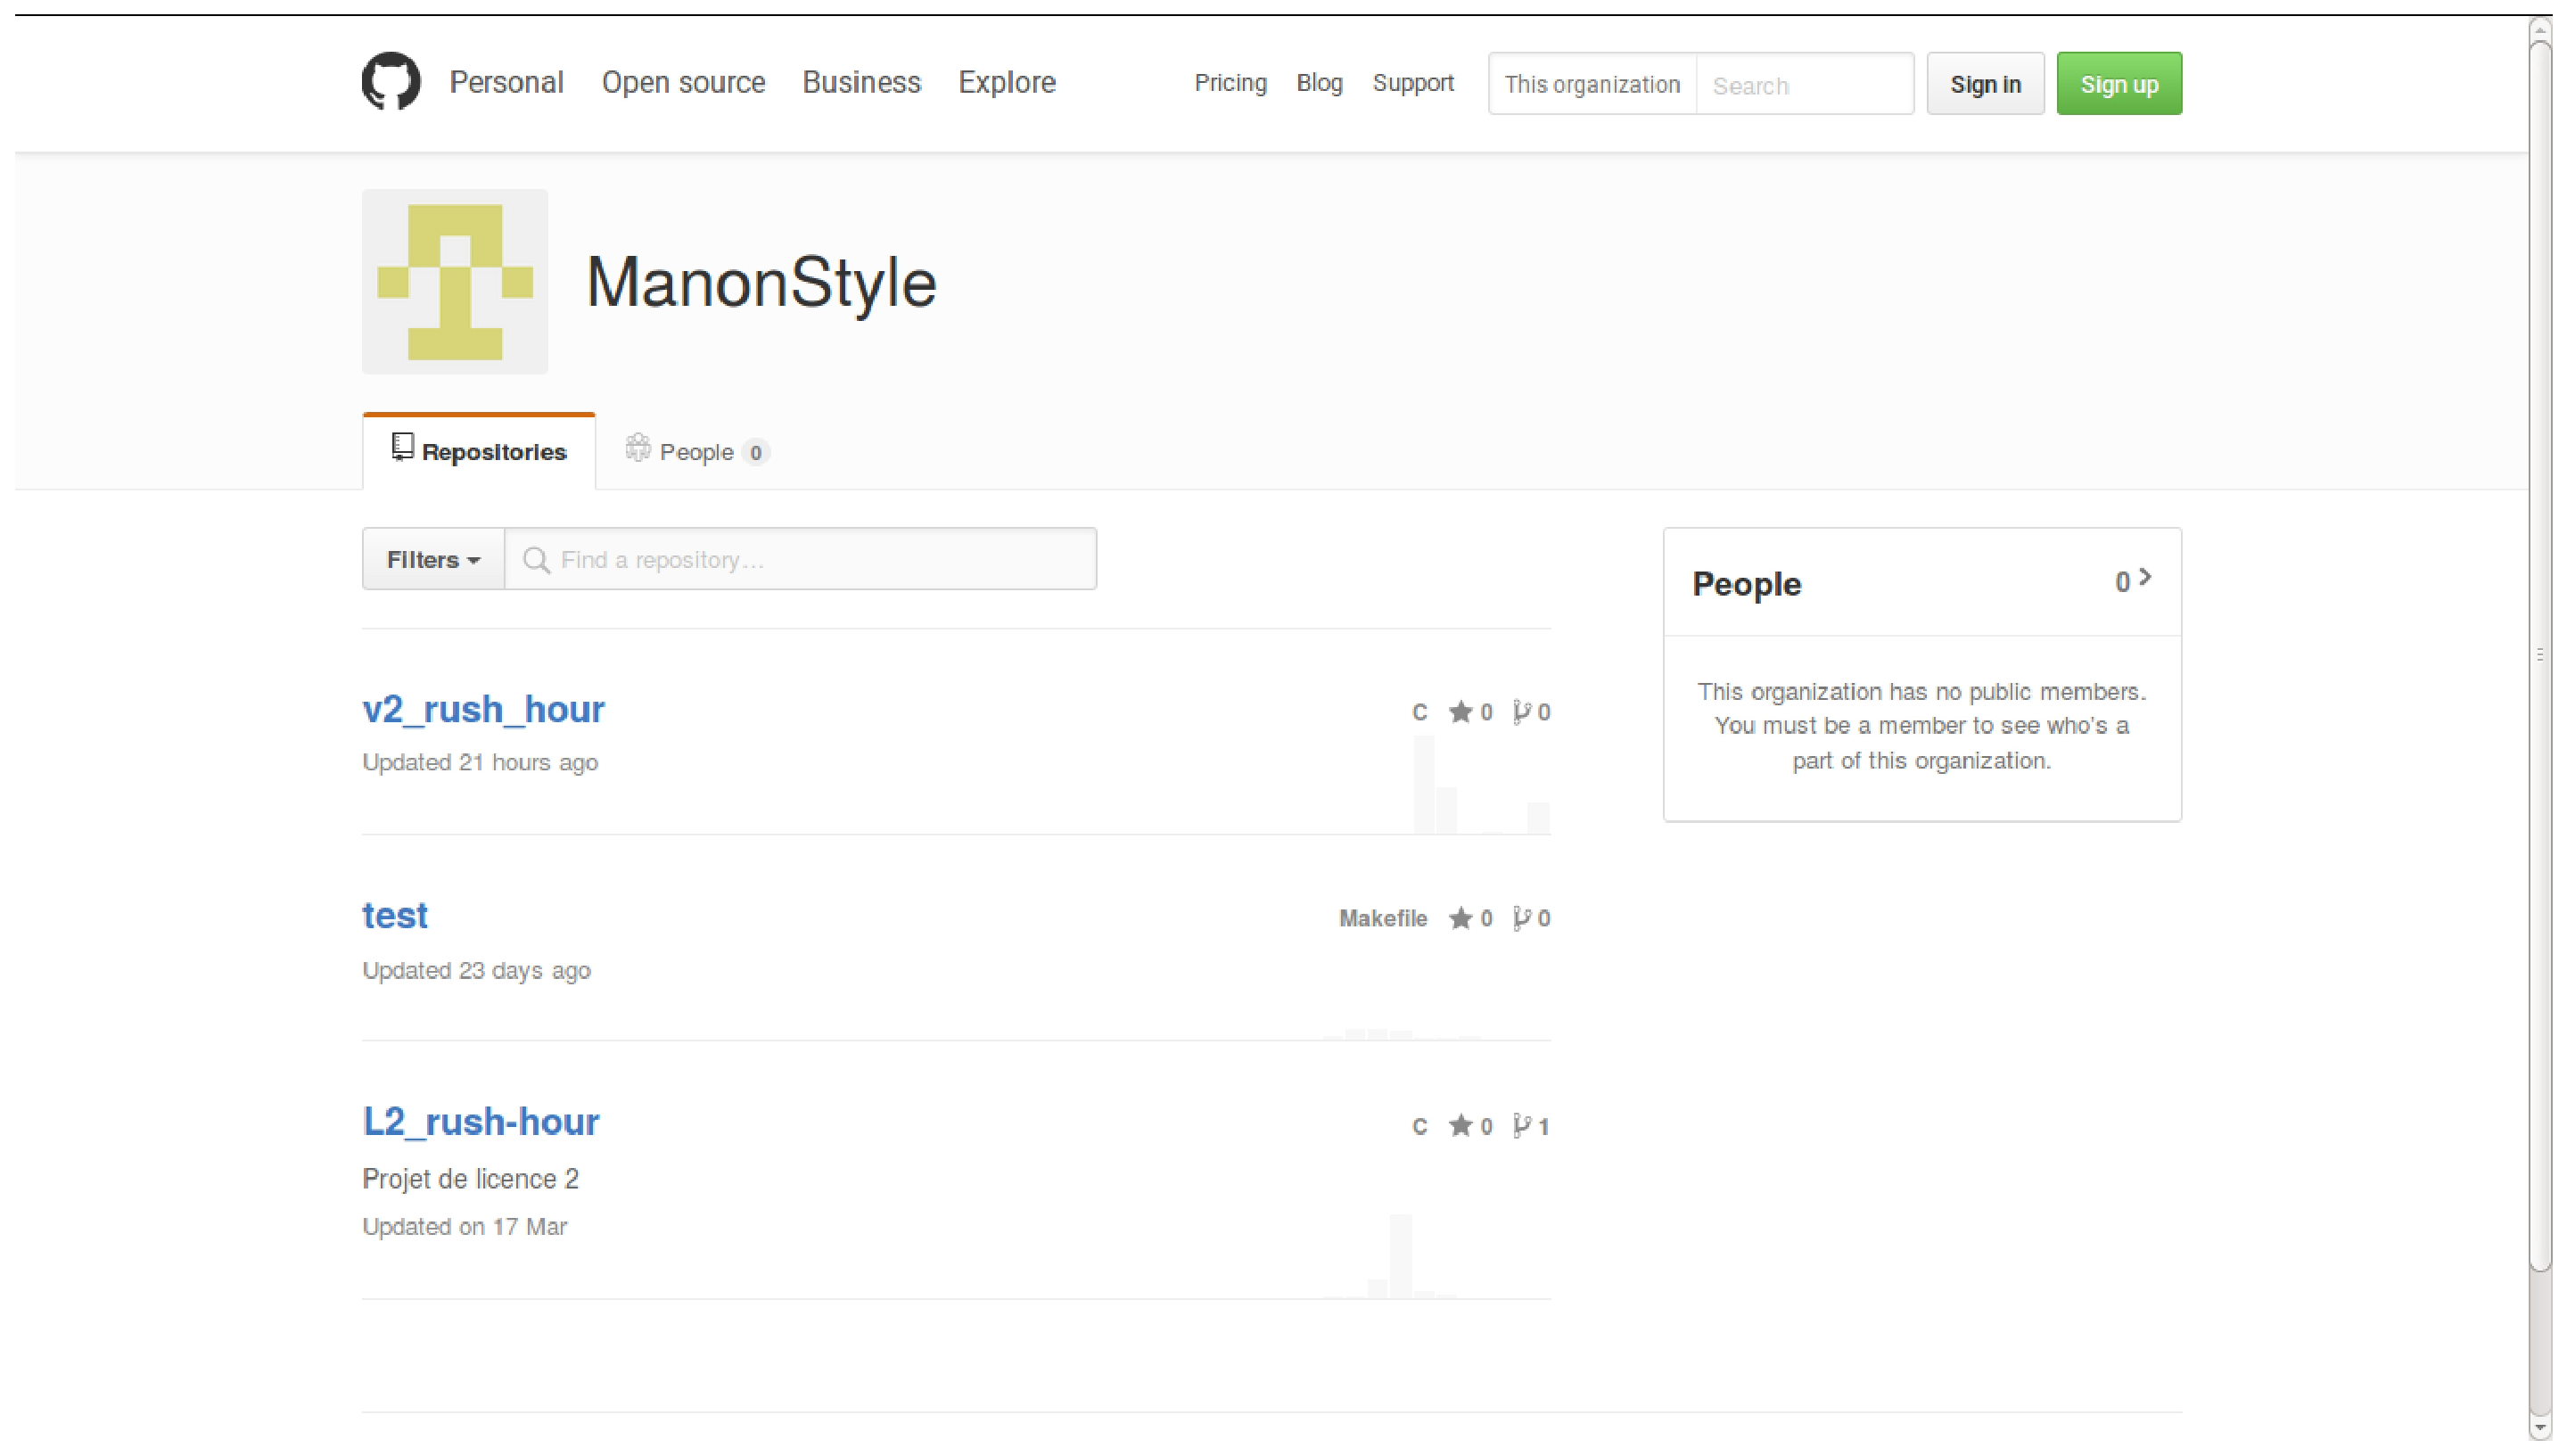
\includegraphics[scale = 0.4, angle = 90]{github.eps}
\end{center}
\caption{\textit{capture d'écran de notre page github : github.com/ManonStyle/}}
\label{github}
\end{figure}

\begin{figure}
\begin{center}
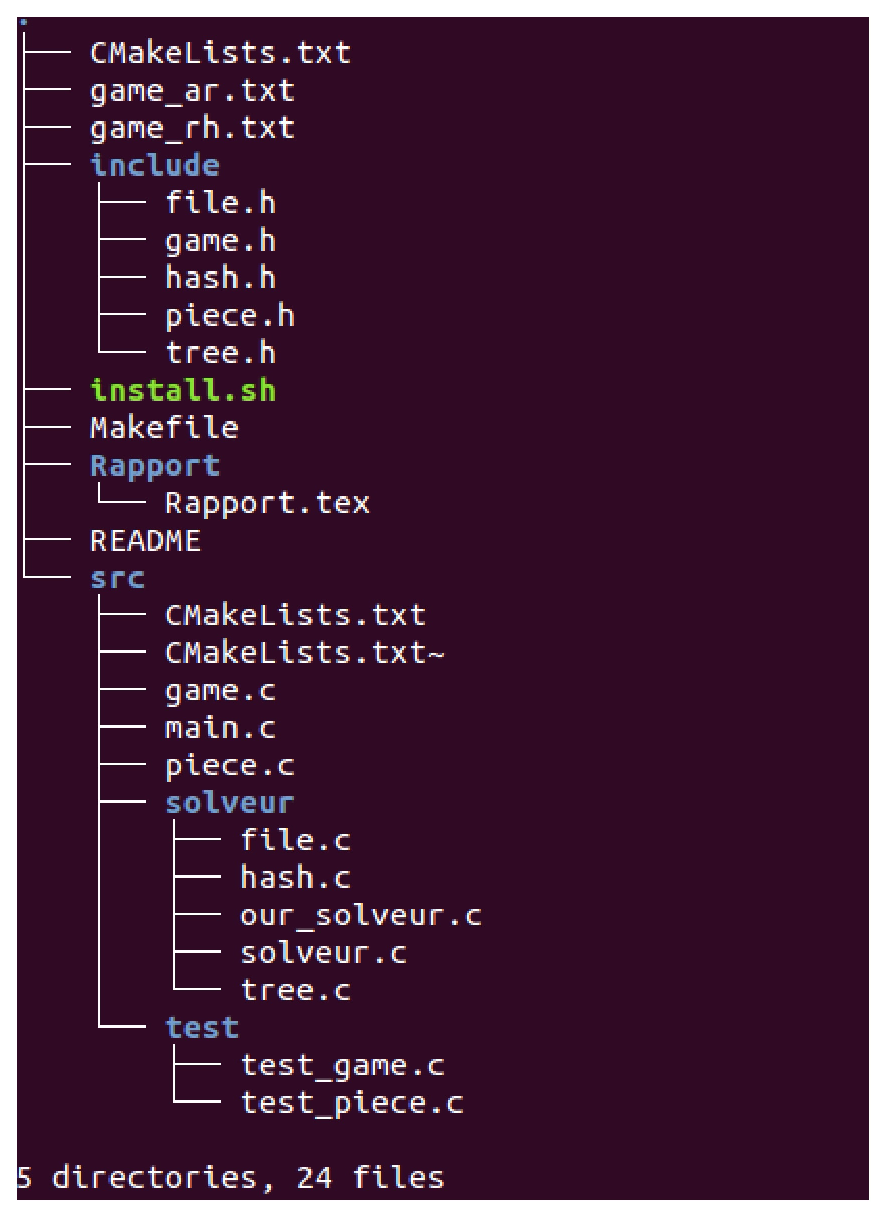
\includegraphics[scale = 1]{structure.eps}
\end{center}
\caption{\textit{capture d'écran de l'arborescence du projet}}
\label{arbor}
\end{figure}

\begin{figure}
\begin{center}
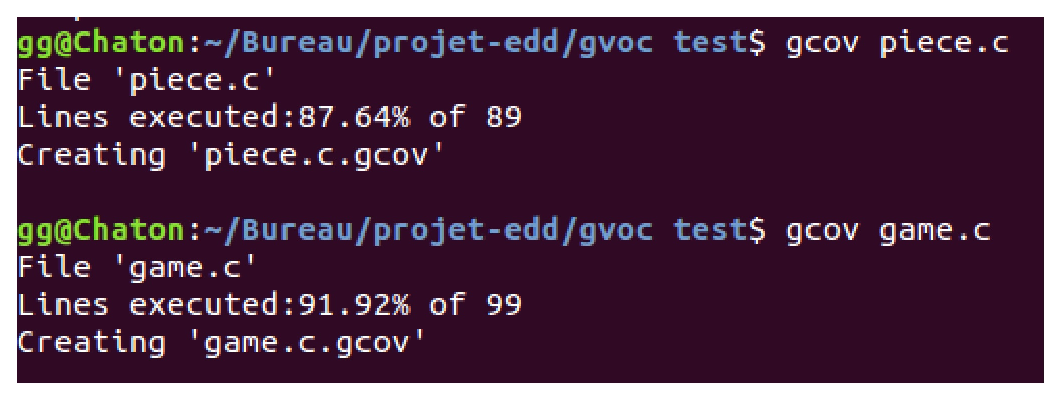
\includegraphics[scale = 0.85]{gcov_terminal.eps}
\end{center}
\caption{\textit{couverture de code des fichiers piece.c et game.c}}
\label{terminal}
\end{figure}

%fin du rapport
\end{document}


%gcov à insérer?
%insérer tuto github
